\subsection{Marketing} \label{marketing_manual}

%Janine 
Now that you have already hired employees, bought components, manufactured products and also delivered them, you have probably wondered how to advertise them and how to communicate with your customers. It's easy, just switch to the marketing view. This includes external communication, legal topics and market research.
Screenshot \ref{fig:marketing_view} shows the marketing view of the current Capitalism X prototype.

\begin{figure}
    \centering
    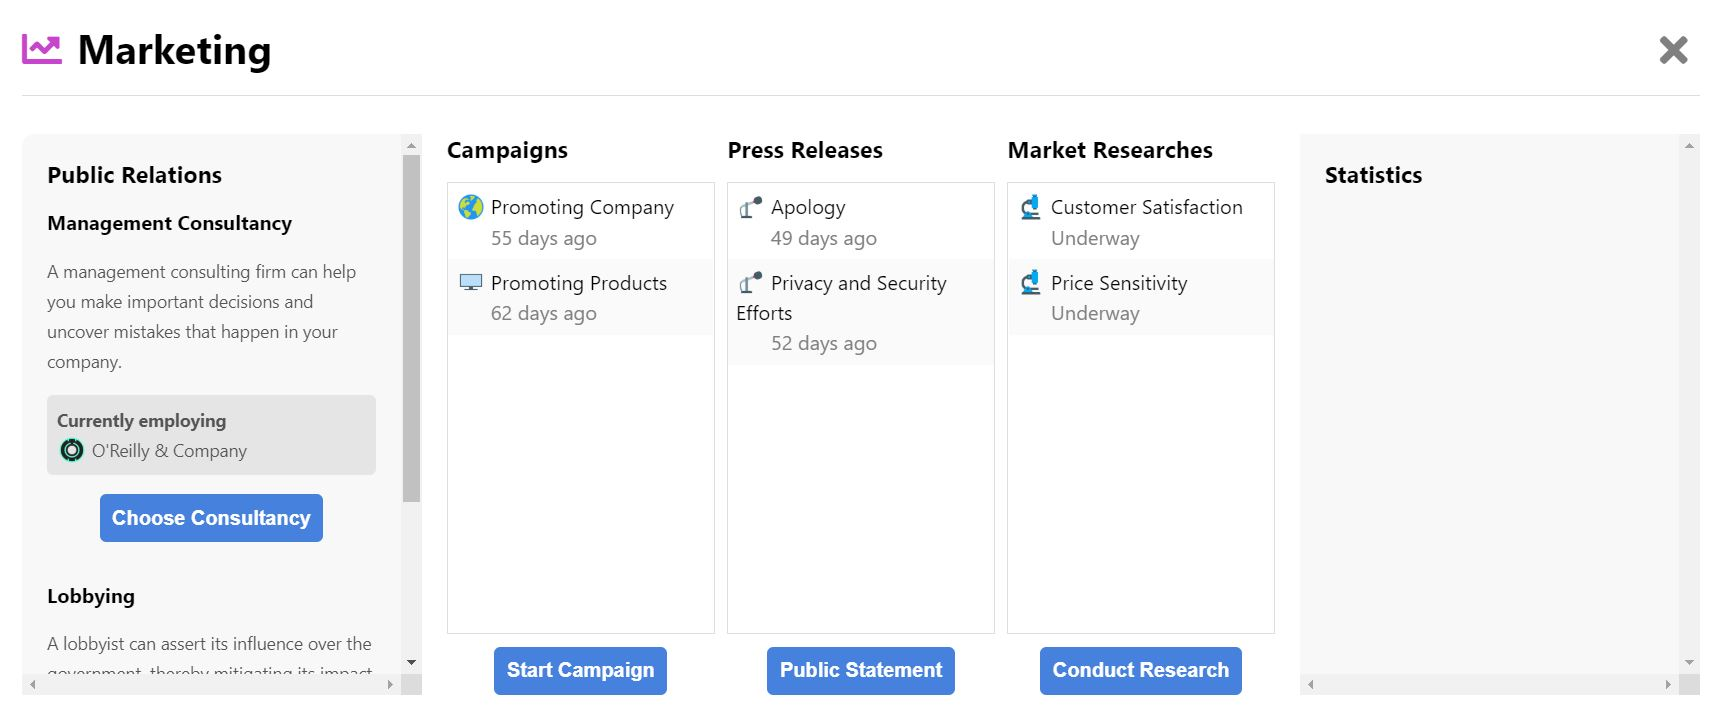
\includegraphics [width=\textwidth]{images/marketing_view.JPG}
    \caption{Marketing View}
    \label{fig:marketing_view}
\end{figure}

%INSERT AT LEAST ONE SCREENSHOT!!!
If you want to advertise products or put your company in the right light, you can do this through campaigns and press releases. You have three different media at your disposal to carry out a marketing campaign: newspapers, television and online.You have three different media at your disposal to carry out a marketing campaign: magazines, television and online. These differ in their reach and also in the costs you have to pay. This is how an online campaign reaches the most customers but also costs you the most. Possible campaigns are: promote a green image, Corporate Social Responsibility (\gls{CSR}) campaign, promoting the company itself, and many more.
In addition to the various campaigns, you can also publish press releases in the marketing view. Press releases can help you to calm the population of CapitalismX after negative situations. If you manage to do this, you can mitigate the impact of external events. Of course, not all press releases are always effective, so make sure they are appropriate. 
For example, you can assure your customers that their data will be handled with care in your company or apologize for inappropriate actions.

In addition to communicating with the population, you can also conduct surveys among them. Click on the 'Conduct Research' button to select the report you want at the end. You have the possibility to carry out the market research yourself or to commission a market research institute with it. If you do it yourself, you can even choose how the actual customer survey is to be conducted. For example, an oral survey is more expensive than an online one, but yields immediate results.  By contrast, an online survey takes longer, which can cause the data to be slightly out of date.

You can basically choose between three reports, a price sensitivity analysis, a customer satisfaction analysis and an overview of various market statistics. The price sensitivity analysis shows you how the buying behaviour of your customers changes when you increase or decrease the price. All other influencing factors are kept constant. The customer satisfaction analysis tells you how satisfied your customers are with your individual products as well as with your company as a whole. The general market analysis shows you a series of market key figures for your products at a glance. 

If you feel that you need help managing your business, or if you just want to be more successful, you can hire either a lobbyist or a business consultancy. The lobbyist will positively help you with the government and try to support you in achieving your goals. 
A management consultancy will take a closer look at your business and try to find areas where you can improve your performance in order to become even more successful.